\documentclass[twoside]{book}

% Packages required by doxygen
\usepackage{fixltx2e}
\usepackage{calc}
\usepackage{doxygen}
\usepackage[export]{adjustbox} % also loads graphicx
\usepackage{graphicx}
\usepackage[utf8]{inputenc}
\usepackage{makeidx}
\usepackage{multicol}
\usepackage{multirow}
\PassOptionsToPackage{warn}{textcomp}
\usepackage{textcomp}
\usepackage[nointegrals]{wasysym}
\usepackage[table]{xcolor}

% Font selection
\usepackage[T1]{fontenc}
\usepackage[scaled=.90]{helvet}
\usepackage{courier}
\usepackage{amssymb}
\usepackage{sectsty}
\renewcommand{\familydefault}{\sfdefault}
\allsectionsfont{%
  \fontseries{bc}\selectfont%
  \color{darkgray}%
}
\renewcommand{\DoxyLabelFont}{%
  \fontseries{bc}\selectfont%
  \color{darkgray}%
}
\newcommand{\+}{\discretionary{\mbox{\scriptsize$\hookleftarrow$}}{}{}}

% Page & text layout
\usepackage{geometry}
\geometry{%
  a4paper,%
  top=2.5cm,%
  bottom=2.5cm,%
  left=2.5cm,%
  right=2.5cm%
}
\tolerance=750
\hfuzz=15pt
\hbadness=750
\setlength{\emergencystretch}{15pt}
\setlength{\parindent}{0cm}
\setlength{\parskip}{3ex plus 2ex minus 2ex}
\makeatletter
\renewcommand{\paragraph}{%
  \@startsection{paragraph}{4}{0ex}{-1.0ex}{1.0ex}{%
    \normalfont\normalsize\bfseries\SS@parafont%
  }%
}
\renewcommand{\subparagraph}{%
  \@startsection{subparagraph}{5}{0ex}{-1.0ex}{1.0ex}{%
    \normalfont\normalsize\bfseries\SS@subparafont%
  }%
}
\makeatother

% Headers & footers
\usepackage{fancyhdr}
\pagestyle{fancyplain}
\fancyhead[LE]{\fancyplain{}{\bfseries\thepage}}
\fancyhead[CE]{\fancyplain{}{}}
\fancyhead[RE]{\fancyplain{}{\bfseries\leftmark}}
\fancyhead[LO]{\fancyplain{}{\bfseries\rightmark}}
\fancyhead[CO]{\fancyplain{}{}}
\fancyhead[RO]{\fancyplain{}{\bfseries\thepage}}
\fancyfoot[LE]{\fancyplain{}{}}
\fancyfoot[CE]{\fancyplain{}{}}
\fancyfoot[RE]{\fancyplain{}{\bfseries\scriptsize Generated by Doxygen }}
\fancyfoot[LO]{\fancyplain{}{\bfseries\scriptsize Generated by Doxygen }}
\fancyfoot[CO]{\fancyplain{}{}}
\fancyfoot[RO]{\fancyplain{}{}}
\renewcommand{\footrulewidth}{0.4pt}
\renewcommand{\chaptermark}[1]{%
  \markboth{#1}{}%
}
\renewcommand{\sectionmark}[1]{%
  \markright{\thesection\ #1}%
}

% Indices & bibliography
\usepackage{natbib}
\usepackage[titles]{tocloft}
\setcounter{tocdepth}{3}
\setcounter{secnumdepth}{5}
\makeindex

% Hyperlinks (required, but should be loaded last)
\usepackage{ifpdf}
\ifpdf
  \usepackage[pdftex,pagebackref=true]{hyperref}
\else
  \usepackage[ps2pdf,pagebackref=true]{hyperref}
\fi
\hypersetup{%
  colorlinks=true,%
  linkcolor=blue,%
  citecolor=blue,%
  unicode%
}

% Custom commands
\newcommand{\clearemptydoublepage}{%
  \newpage{\pagestyle{empty}\cleardoublepage}%
}

\usepackage{caption}
\captionsetup{labelsep=space,justification=centering,font={bf},singlelinecheck=off,skip=4pt,position=top}

%===== C O N T E N T S =====

\begin{document}

% Titlepage & ToC
\hypersetup{pageanchor=false,
             bookmarksnumbered=true,
             pdfencoding=unicode
            }
\pagenumbering{alph}
\begin{titlepage}
\vspace*{7cm}
\begin{center}%
{\Large Excellentea \\[1ex]\large 1.\+0 }\\
\vspace*{1cm}
{\large Generated by Doxygen 1.8.15}\\
\end{center}
\end{titlepage}
\clearemptydoublepage
\pagenumbering{roman}
\tableofcontents
\clearemptydoublepage
\pagenumbering{arabic}
\hypersetup{pageanchor=true}

%--- Begin generated contents ---
\chapter{Guidelines}
\label{md_CONTRIBUTING}
\Hypertarget{md_CONTRIBUTING}
This file will contain the main guidelines for contribution to the project. 
\chapter{R\+E\+A\+D\+ME}
\label{md_README}
\Hypertarget{md_README}


\section*{Description}

Excellentea is an automatic tea maker. The user can operate the machine remotely through an online interface. In other words, you can order your tea, by chosing from several modes, as you leave work and find it ready when you get home. It also comes with the option of controlling the machine using control buttons and an L\+CD display.

\section*{Usage}

\subsection*{Installation}

Clone the repository to your Raspberry Pi and run the following commands\+:


\begin{DoxyCode}
./configure
make
make install
\end{DoxyCode}
 The program can then be started by running the command


\begin{DoxyCode}
excellentea
\end{DoxyCode}
 from the terminal.

\subsection*{User operation}


\begin{DoxyEnumerate}
\item Load your cup with water
\item Load your tea infuser with the tea of your choice
\item Activate the tea maker from the online user interface
\item Choose the brewing mode of your tea
\item Wait...tea is ready\+:)
\end{DoxyEnumerate}

\section*{Hardware}

\subsection*{Key components}


\begin{DoxyItemize}
\item 1 Raspberry PI microcontroller board (tested on version 3 Model B)
\item 1 \mbox{\hyperlink{classStepper}{Stepper}} motor (M\+I\+K\+R\+O\+E-\/1530)
\item 1 Digital temperature sensor (ds18b20)
\item 12V DC power supply
\item 1 heating element (12V) (B004\+O8\+B\+G\+XE)
\item 1 tea infuser
\item 1 reed float sensor (59630)
\item 2 18-\/pin through hole socket (E\+D18\+DT)
\item 2 Darlington transistor array (U\+L\+N2803A)
\item L\+CD
\item 2 N-\/channel logic-\/level M\+O\+S\+F\+ET (F\+Q\+P30\+N06L)
\item M\+O\+S\+F\+ET heat sink (507222\+B00000G)
\end{DoxyItemize}

\subsection*{Additional components}

The project also requires standard passive components (e.\+g. resistors), prototyping tools (e.\+g. breadboard/pcb) and materials for the encasing. See the \href{Main.sch}{\tt circuit schematics} for details.

\subsection*{Protocol}

The digital temperature sensor \mbox{\hyperlink{classDS18B20}{D\+S18\+B20}} communicates with the board through a 1-\/wire protocol on pin 7 (B\+C\+M4). The reed float sensor only outputs two-\/states so a communication protocol is not required.

\subsection*{Prerequisites}

The raspberry PI must be connected to the internet for remote access.

\section*{Software}

\subsection*{Flow diagram}



\section*{Authors}


\begin{DoxyItemize}
\item \href{https://github.com/andreaspanou}{\tt {\bfseries Andrea Spanou}} -\/ {\itshape Initial work}
\item \href{https://github.com/CiaranAnthony}{\tt {\bfseries Ciaran Mc\+Geady}} -\/ {\itshape Initial work}
\item \href{https://github.com/SimoneMarcigaglia}{\tt {\bfseries Simone Marcigaglia}} -\/ {\itshape Initial work}
\end{DoxyItemize}

See also the list of \href{https://github.com/GlasgowTeam3RTEP/ExcellenTea/contributors}{\tt contributors} who participated in this project.

\section*{Contributing}

Please read \mbox{\hyperlink{md_CONTRIBUTING}{C\+O\+N\+T\+R\+I\+B\+U\+T\+I\+NG.md}} for details on our code of conduct, and the process for submitting pull requests to us.

\section*{License}

This project is licensed under the M\+IT License -\/ see the \mbox{[}L\+I\+C\+E\+N\+SE\mbox{]}(L\+I\+C\+E\+N\+SE) file for details.

\section*{Acknowledgments}

We would like to thank the weather in Glasgow for making us think about tea all the time. 
\chapter{Hierarchical Index}
\section{Class Hierarchy}
This inheritance list is sorted roughly, but not completely, alphabetically\+:\begin{DoxyCompactList}
\item \contentsline{section}{sensor}{\pageref{classsensor}}{}
\begin{DoxyCompactList}
\item \contentsline{section}{ds18b20}{\pageref{classds18b20}}{}
\end{DoxyCompactList}
\item \contentsline{section}{stepper}{\pageref{classstepper}}{}
\item \contentsline{section}{tea}{\pageref{classtea}}{}
\end{DoxyCompactList}

\chapter{Class Index}
\section{Class List}
Here are the classes, structs, unions and interfaces with brief descriptions\+:\begin{DoxyCompactList}
\item\contentsline{section}{\mbox{\hyperlink{classActuator}{Actuator}} \\*A general class for external loads }{\pageref{classActuator}}{}
\item\contentsline{section}{\mbox{\hyperlink{classBrewTimer}{Brew\+Timer}} }{\pageref{classBrewTimer}}{}
\item\contentsline{section}{\mbox{\hyperlink{classControllerThread}{Controller\+Thread}} }{\pageref{classControllerThread}}{}
\item\contentsline{section}{\mbox{\hyperlink{classCppThread}{Cpp\+Thread}} \\*G\+NU G\+E\+N\+E\+R\+AL P\+U\+B\+L\+IC L\+I\+C\+E\+N\+SE Version 3, 29 June 2007 }{\pageref{classCppThread}}{}
\item\contentsline{section}{\mbox{\hyperlink{classCppTimer}{Cpp\+Timer}} }{\pageref{classCppTimer}}{}
\item\contentsline{section}{\mbox{\hyperlink{classDS18B20}{D\+S18\+B20}} \\*Class for the digital temperature sensor \mbox{\hyperlink{classDS18B20}{D\+S18\+B20}} }{\pageref{classDS18B20}}{}
\item\contentsline{section}{\mbox{\hyperlink{classSensor}{Sensor}} \\*A general class for simple H\+I\+G\+H/\+L\+OW sensors }{\pageref{classSensor}}{}
\item\contentsline{section}{\mbox{\hyperlink{classStepper}{Stepper}} \\*A class to control stepper motors }{\pageref{classStepper}}{}
\item\contentsline{section}{\mbox{\hyperlink{classTea}{Tea}} \\*A class defining a type of tea by its brewing time and temperature }{\pageref{classTea}}{}
\item\contentsline{section}{\mbox{\hyperlink{classWebThread}{Web\+Thread}} \\*A thread that handles the web interface }{\pageref{classWebThread}}{}
\end{DoxyCompactList}

\chapter{Class Documentation}
\hypertarget{classds18b20}{}\section{ds18b20 Class Reference}
\label{classds18b20}\index{ds18b20@{ds18b20}}


Class for the digital temperature sensor D\+S18\+B20.  




{\ttfamily \#include $<$ds18b20.\+h$>$}



Inheritance diagram for ds18b20\+:\nopagebreak
\begin{figure}[H]
\begin{center}
\leavevmode
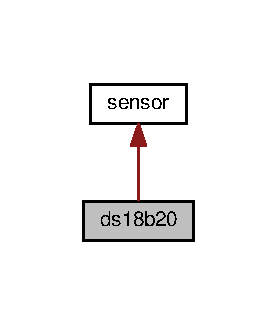
\includegraphics[width=133pt]{classds18b20__inherit__graph}
\end{center}
\end{figure}


Collaboration diagram for ds18b20\+:\nopagebreak
\begin{figure}[H]
\begin{center}
\leavevmode
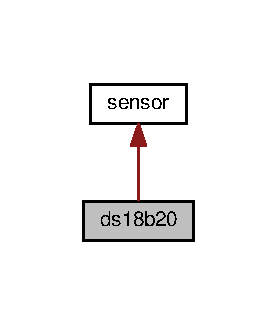
\includegraphics[width=133pt]{classds18b20__coll__graph}
\end{center}
\end{figure}
\subsection*{Public Member Functions}
\begin{DoxyCompactItemize}
\item 
\mbox{\hyperlink{classds18b20_a2feec12ddec6572d29db8b0fe7181bab}{ds18b20}} (short G\+P\+IO, std\+::string dev\+\_\+id)
\begin{DoxyCompactList}\small\item\em Class constructor. \end{DoxyCompactList}\item 
void \mbox{\hyperlink{classds18b20_a222d770b98aa7c0d6ae27da9756c8979}{initialise}} ()
\begin{DoxyCompactList}\small\item\em Initialisation procedure. \end{DoxyCompactList}\item 
double \mbox{\hyperlink{classds18b20_a479caadfcbf4b1d0fd0867a440900e7d}{read\+Temp}} ()
\begin{DoxyCompactList}\small\item\em Read the temperature from the sensor. \end{DoxyCompactList}\end{DoxyCompactItemize}


\subsection{Detailed Description}
Class for the digital temperature sensor D\+S18\+B20. 



\subsection{Constructor \& Destructor Documentation}
\mbox{\Hypertarget{classds18b20_a2feec12ddec6572d29db8b0fe7181bab}\label{classds18b20_a2feec12ddec6572d29db8b0fe7181bab}} 
\index{ds18b20@{ds18b20}!ds18b20@{ds18b20}}
\index{ds18b20@{ds18b20}!ds18b20@{ds18b20}}
\subsubsection{\texorpdfstring{ds18b20()}{ds18b20()}}
{\footnotesize\ttfamily ds18b20\+::ds18b20 (\begin{DoxyParamCaption}\item[{short}]{G\+P\+IO,  }\item[{std\+::string}]{dev\+\_\+id }\end{DoxyParamCaption})}



Class constructor. 

Build a temperature sensor object with the pin number and the unique device ID. 
\begin{DoxyParams}{Parameters}
{\em G\+P\+IO} & pin number (wiring\+Pi convention) \\
\hline
{\em dev\+\_\+id} & device ID on the bus as a string \\
\hline
\end{DoxyParams}


\subsection{Member Function Documentation}
\mbox{\Hypertarget{classds18b20_a222d770b98aa7c0d6ae27da9756c8979}\label{classds18b20_a222d770b98aa7c0d6ae27da9756c8979}} 
\index{ds18b20@{ds18b20}!initialise@{initialise}}
\index{initialise@{initialise}!ds18b20@{ds18b20}}
\subsubsection{\texorpdfstring{initialise()}{initialise()}}
{\footnotesize\ttfamily void ds18b20\+::initialise (\begin{DoxyParamCaption}{ }\end{DoxyParamCaption})\hspace{0.3cm}{\ttfamily [virtual]}}



Initialisation procedure. 

Activates the one-\/wire interface from the Raspberry PI. 

Reimplemented from \mbox{\hyperlink{classsensor_ae1073389f46dd119e2f421a894b7d781}{sensor}}.

\mbox{\Hypertarget{classds18b20_a479caadfcbf4b1d0fd0867a440900e7d}\label{classds18b20_a479caadfcbf4b1d0fd0867a440900e7d}} 
\index{ds18b20@{ds18b20}!read\+Temp@{read\+Temp}}
\index{read\+Temp@{read\+Temp}!ds18b20@{ds18b20}}
\subsubsection{\texorpdfstring{read\+Temp()}{readTemp()}}
{\footnotesize\ttfamily double ds18b20\+::read\+Temp (\begin{DoxyParamCaption}{ }\end{DoxyParamCaption})}



Read the temperature from the sensor. 

Request the temperature value from the sensor and returns a double precision value. 

The documentation for this class was generated from the following files\+:\begin{DoxyCompactItemize}
\item 
sensors/ds18b20.\+h\item 
sensors/ds18b20.\+cpp\end{DoxyCompactItemize}

\hypertarget{classsensor}{}\section{sensor Class Reference}
\label{classsensor}\index{sensor@{sensor}}


A general class for simple H\+I\+G\+H/\+L\+OW sensors.  




{\ttfamily \#include $<$sensor.\+h$>$}



Inheritance diagram for sensor\+:\nopagebreak
\begin{figure}[H]
\begin{center}
\leavevmode
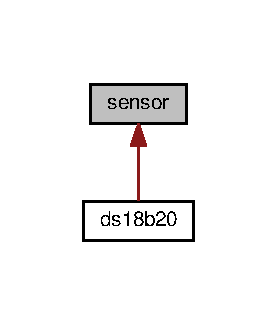
\includegraphics[width=133pt]{classsensor__inherit__graph}
\end{center}
\end{figure}
\subsection*{Public Member Functions}
\begin{DoxyCompactItemize}
\item 
\mbox{\hyperlink{classsensor_a3341a98b9c6b4f0e0234f205941f4342}{sensor}} (short G\+P\+IO)
\begin{DoxyCompactList}\small\item\em Class constructor. \end{DoxyCompactList}\item 
\mbox{\Hypertarget{classsensor_ae1073389f46dd119e2f421a894b7d781}\label{classsensor_ae1073389f46dd119e2f421a894b7d781}} 
virtual void \mbox{\hyperlink{classsensor_ae1073389f46dd119e2f421a894b7d781}{initialise}} ()
\begin{DoxyCompactList}\small\item\em Initialisation procedure with wiring\+Pi library. \end{DoxyCompactList}\item 
\mbox{\Hypertarget{classsensor_a111c7b59fb50d61c0e44e689b8eb94f9}\label{classsensor_a111c7b59fb50d61c0e44e689b8eb94f9}} 
bool \mbox{\hyperlink{classsensor_a111c7b59fb50d61c0e44e689b8eb94f9}{read\+Status}} ()
\begin{DoxyCompactList}\small\item\em Reads boolean status of the sensor. \end{DoxyCompactList}\end{DoxyCompactItemize}
\subsection*{Protected Attributes}
\begin{DoxyCompactItemize}
\item 
\mbox{\Hypertarget{classsensor_a4fb74b2b7aedb1554825444387c0d017}\label{classsensor_a4fb74b2b7aedb1554825444387c0d017}} 
short {\bfseries pin}
\end{DoxyCompactItemize}


\subsection{Detailed Description}
A general class for simple H\+I\+G\+H/\+L\+OW sensors. 

\subsection{Constructor \& Destructor Documentation}
\mbox{\Hypertarget{classsensor_a3341a98b9c6b4f0e0234f205941f4342}\label{classsensor_a3341a98b9c6b4f0e0234f205941f4342}} 
\index{sensor@{sensor}!sensor@{sensor}}
\index{sensor@{sensor}!sensor@{sensor}}
\subsubsection{\texorpdfstring{sensor()}{sensor()}}
{\footnotesize\ttfamily sensor\+::sensor (\begin{DoxyParamCaption}\item[{short}]{G\+P\+IO }\end{DoxyParamCaption})}



Class constructor. 


\begin{DoxyParams}{Parameters}
{\em G\+P\+IO} & Raspberry pi pin connected to the sensor. \\
\hline
\end{DoxyParams}


The documentation for this class was generated from the following files\+:\begin{DoxyCompactItemize}
\item 
sensors/sensor.\+h\item 
sensors/sensor.\+cpp\end{DoxyCompactItemize}

\hypertarget{classstepper}{}\section{stepper Class Reference}
\label{classstepper}\index{stepper@{stepper}}
\subsection*{Public Member Functions}
\begin{DoxyCompactItemize}
\item 
\mbox{\Hypertarget{classstepper_a294329374cfa14bc65faef71fcf0c780}\label{classstepper_a294329374cfa14bc65faef71fcf0c780}} 
void {\bfseries initialize} ()
\item 
\mbox{\Hypertarget{classstepper_aaa1c9583e55db54218231560eeddadb2}\label{classstepper_aaa1c9583e55db54218231560eeddadb2}} 
void {\bfseries spin} (int speed, int revolutions, bool direction)
\item 
\mbox{\Hypertarget{classstepper_aceb54bf5d1838efdab59b04132ad3086}\label{classstepper_aceb54bf5d1838efdab59b04132ad3086}} 
{\bfseries stepper} (short A1, short A2, short B1, short B2, int steps)
\end{DoxyCompactItemize}


The documentation for this class was generated from the following files\+:\begin{DoxyCompactItemize}
\item 
stepper/stepper.\+h\item 
stepper/stepper.\+cpp\end{DoxyCompactItemize}

\hypertarget{classtea}{}\section{tea Class Reference}
\label{classtea}\index{tea@{tea}}
\subsection*{Public Member Functions}
\begin{DoxyCompactItemize}
\item 
\mbox{\Hypertarget{classtea_a6853c9899596abea3121aae76b12e5f6}\label{classtea_a6853c9899596abea3121aae76b12e5f6}} 
void {\bfseries set\+Brew\+Temperature} (double temp)
\item 
\mbox{\Hypertarget{classtea_aa541720b90b31274c3bba3e77d765c81}\label{classtea_aa541720b90b31274c3bba3e77d765c81}} 
void {\bfseries set\+Brew\+Time} (double time)
\item 
\mbox{\Hypertarget{classtea_a8a83c91eb834c18d646e048e82a8528b}\label{classtea_a8a83c91eb834c18d646e048e82a8528b}} 
double {\bfseries get\+Brew\+Temperature} ()
\item 
\mbox{\Hypertarget{classtea_a550ccb4846b555ed1717e7e8373d8a25}\label{classtea_a550ccb4846b555ed1717e7e8373d8a25}} 
double {\bfseries get\+Brew\+Time} ()
\item 
\mbox{\Hypertarget{classtea_ae5f444d5215b49aae039b46a47ad908f}\label{classtea_ae5f444d5215b49aae039b46a47ad908f}} 
{\bfseries tea} (double brew\+\_\+temp, double brew\+\_\+time)
\end{DoxyCompactItemize}


The documentation for this class was generated from the following files\+:\begin{DoxyCompactItemize}
\item 
tea/tea.\+h\item 
tea/tea.\+cpp\end{DoxyCompactItemize}

%--- End generated contents ---

% Index
\backmatter
\newpage
\phantomsection
\clearemptydoublepage
\addcontentsline{toc}{chapter}{Index}
\printindex

\end{document}
